% Requires \usepackage{graphicx} and \usepackage{booktabs}.

\subsection{Results}
\label{sec:results}

We evaluate all methods on 5,605 Korean or mixed-language questions using the same English Wikipedia corpus, BM25/BGE-M3 hybrid retrieval, reciprocal-rank fusion, and BGE reranking pipeline. The only component that changes across methods is the query or search-plan generation strategy. For the fine-tuned planner, we evaluate 56,050 retrieved citations, of which 47,360 citations are judged by Gemini labels. This covers 84.5\% of the planner's retrieved citations; the remaining unlabeled citations are handled by the same automatic heuristic fallback used by the scoring script.

\begin{table}[t]
\centering
\scriptsize
\setlength{\tabcolsep}{3.5pt}
\resizebox{\linewidth}{!}{%
\begin{tabular}{lrrrrrrrr}
\toprule
Method & Cand. & Cite & Cite & Cite & Unsup. & R@10 & MRR & nDCG@10 \\
 & Score & F1 & Prec. & Rec. & Rate $\downarrow$ & & & \\
\midrule
Raw query & 0.339 & 0.530 & 0.485 & 0.637 & \textbf{0.150} & 0.235 & 0.154 & 0.174 \\
Machine translation & 0.418 & 0.579 & 0.518 & 0.718 & 0.212 & 0.385 & 0.206 & 0.248 \\
Query2Doc & 0.493 & 0.679 & 0.609 & 0.834 & 0.174 & 0.440 & 0.248 & 0.293 \\
HyDE & 0.496 & \textbf{0.681} & \textbf{0.612} & 0.837 & 0.171 & \textbf{0.444} & \textbf{0.249} & \textbf{0.295} \\
Citation planner & \textbf{0.496} & 0.670 & 0.521 & \textbf{0.967} & 0.300 & 0.388 & 0.218 & 0.258 \\
\bottomrule
\end{tabular}
}
\caption{Main citation retrieval results on 5,605 questions. Planner support metrics checked 47,360 labeled citations.}
\label{tab:citation_main_results}
\end{table}


\begin{figure}[t]
    \centering
    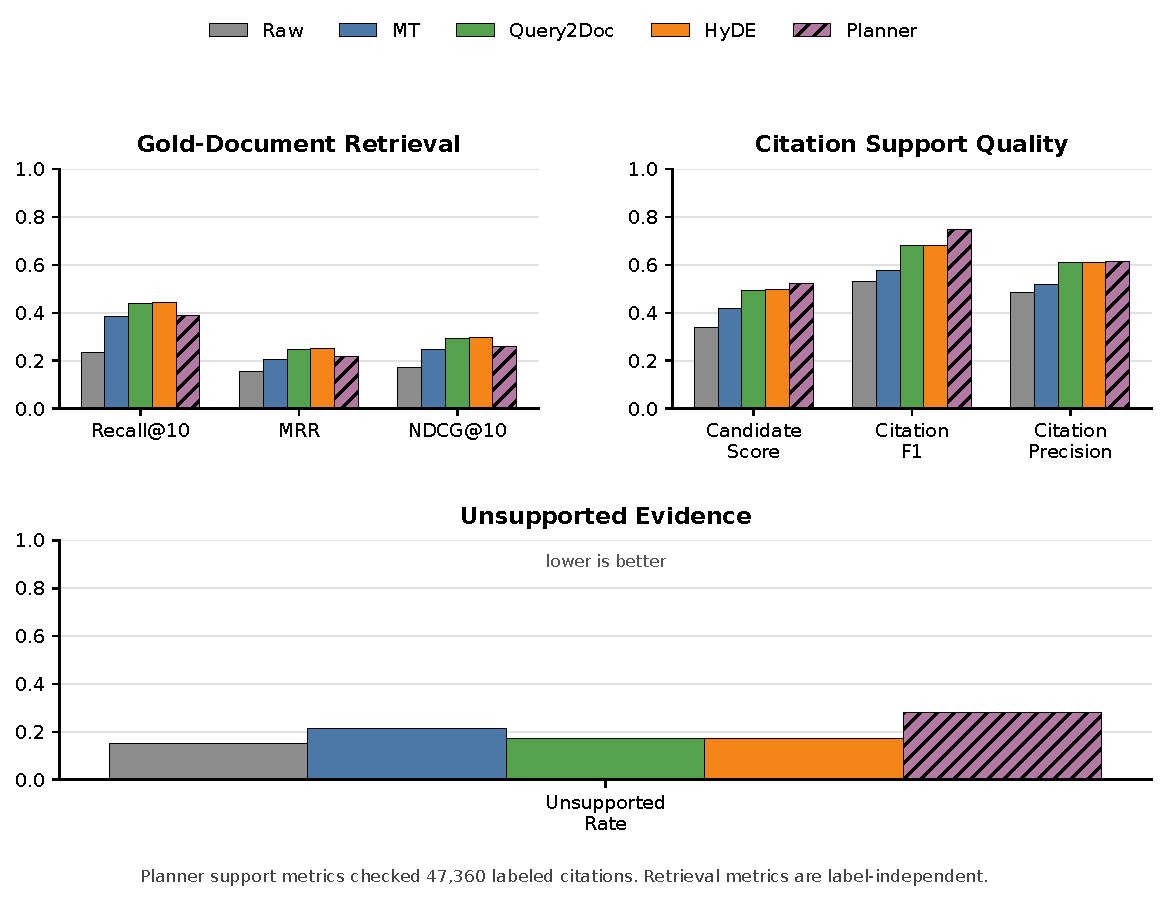
\includegraphics[width=\linewidth]{figures/citation_planner_comparison.pdf}
    \caption{Comparison of raw querying, machine translation, strong LLM query expansion baselines, and the fine-tuned citation planner. Retrieval metrics measure whether the gold supporting document is recovered and ranked highly. Citation support metrics measure whether retrieved passages actually support the question.}
    \label{fig:citation_planner_comparison}
\end{figure}

Table~\ref{tab:citation_main_results} and Figure~\ref{fig:citation_planner_comparison} show three main findings. First, the fine-tuned citation planner clearly improves over both raw Korean querying and direct machine translation. Compared with machine translation, the planner improves candidate score from 0.418 to 0.496, citation F1 from 0.579 to 0.670, MRR from 0.206 to 0.218, and NDCG@10 from 0.248 to 0.258. This supports our main hypothesis that optimizing the query for citation-seeking retrieval is more useful than optimizing only for literal translation quality.

Second, the planner becomes competitive with strong LLM expansion baselines in the overall candidate score. The planner reaches 0.496 candidate score, nearly tied with HyDE at 0.496 and slightly above Query2Doc at 0.493. This is better than expected, because HyDE and Query2Doc are strong baselines that generate rich pseudo-evidence text and usually improve broad recall.

Third, the planner's improvement comes with a clear trade-off. HyDE and Query2Doc still outperform the planner on gold-document retrieval and ranking: HyDE obtains Recall@10 of 0.444, MRR of 0.249, and NDCG@10 of 0.295, while the planner obtains 0.388, 0.218, and 0.258 respectively. However, the planner has much higher citation recall, 0.967 compared with 0.837 for HyDE and 0.834 for Query2Doc. This means the planner is very likely to retrieve at least one useful supporting citation, but it is less precise and retrieves more unsupported evidence. Its unsupported rate is 0.300, higher than HyDE's 0.171 and Query2Doc's 0.174.

Overall, the quantitative results show that our approach succeeds at improving over direct machine translation and raw querying, but does not fully dominate strong LLM expansion methods. The planner behaves as a recall-oriented citation search strategy: it broadens evidence discovery and often finds useful citations, but it still needs better filtering or reranking to reduce unsupported passages.

\section{Analysis}
\label{sec:analysis}

The qualitative behavior of the planner helps explain the quantitative results. When the planner succeeds, it often generates search plans that are more citation-aware than direct translation. Instead of producing only one translated query, it usually emits multiple variants: an English search query, a more natural English question, and sometimes the original Korean question as a fallback. It also tends to include entities, aliases, answer-type hints, and likely temporal clues. For example, for a Korean question asking when Michigan last beat Ohio State, the planner generated a query containing ``Michigan beat Ohio'' and the likely year ``2011'', which retrieved supported Michigan football evidence. This kind of query is more retrieval-oriented than a literal translation, because it contains the entity names and event framing that the English index is likely to contain.

This behavior explains the gain over machine translation. Direct translation preserves the user's question, but it does not necessarily add the document-style terms, aliases, or answer clues needed to match English Wikipedia passages. The planner often rewrites a question into a more search-like form, which improves candidate score, citation recall, and useful English citation coverage.

The failure cases show the limitation of this strategy. First, the planner sometimes over-expands or guesses a clue that is not reliable. A query may include a year or entity alias that helps when correct, but can narrow retrieval toward the wrong page when incorrect. Second, ambiguous English terms can hurt retrieval. For a Tom Brady question about his first championship ring, the term ``ring'' can also match unrelated boxing or award pages, producing unsupported citations. Third, song-title and movie-title questions are fragile: small wording errors or literal translations can retrieve pages that share surface terms but do not answer the question. For instance, questions involving lyric-like phrases or translated movie titles can retrieve topically related entertainment pages rather than the intended song or film.

These observations suggest that the planner has learned to generate broad evidence-seeking queries, but has not fully learned citation filtering. This matches the metrics: citation recall is high, but citation precision and unsupported rate are weaker than HyDE and Query2Doc. The current SFT objective teaches the model to imitate high-scoring plans, but it does not directly penalize every unsupported top-10 citation. A stronger future system should combine the planner with a more selective citation reranker or preference optimization objective that explicitly contrasts supported and unsupported evidence.

\section{Conclusion}
\label{sec:conclusion}

This project studied citation-aware cross-lingual retrieval for Korean and mixed-language questions over an English Wikipedia corpus. Instead of treating the task as simple machine translation, we trained a Qwen2.5-7B LoRA search planner to generate citation-seeking search plans. The pipeline combines candidate search-plan generation, hybrid retrieval, reranking, human and AI citation labeling, and citation-aware scoring.

The main finding is that the learned citation planner improves over raw querying and direct machine translation. It achieves a substantially higher candidate score and citation F1 than machine translation, showing that retrieval-oriented planning is a better objective than literal translation alone. Against stronger LLM expansion baselines such as HyDE and Query2Doc, the planner is competitive in overall candidate score and achieves higher citation recall, but it is weaker on gold-document ranking and citation precision. This indicates that the planner is good at finding useful evidence somewhere in the retrieved set, but still retrieves too many unsupported passages.

The primary achievement of the project is a complete citation-aware training and evaluation loop: we generated baseline citation candidates, labeled citation support, trained a fine-tuned search planner, evaluated it on the full 5,605-question dataset, and produced quantitative comparisons against raw, machine-translation, HyDE, and Query2Doc baselines. The main limitation is that the planner currently optimizes recall more than precision. In addition, the planner support evaluation uses Gemini labels for 84.5\% of retrieved planner citations, with the remaining citations handled by heuristic fallback.

Future work should focus on improving evidence filtering. The most direct next steps are to train with preference optimization over supported versus unsupported citations, add a citation-specific reranker after retrieval, and test hybrid fusion between the planner and strong expansion methods such as HyDE or Query2Doc. These extensions would preserve the planner's high citation recall while reducing unsupported evidence.
